\section{Semantic Web}


\subsection{Semi-structured data}

\paragraph{Schemas} define data structures for database. Label the column, add constraint,
\dots But imposing the use of schema on the web might be too rigid and turn into a disadvantage

\paragraph{Semi-structure Data:} data that contains tags, markup, similar to specify the semantic of data valued and to relate different data values e.g. hierarchically. No predefined structure, no schema required (e.g. JSON, XML, ...)

\subsubsection{Schema-less Data}

\paragraph{Benefit:}

\begin{itemize}
\item increased flexibility: dynamically adding or dropping structural elements such as attribute
\item Self-contained data: context (schema information) directly encoded into data
\end{itemize}

\paragraph{Drawback:}

\begin{itemize}
\item Loss of consistency
\item Certain optimizations not feasible: in the absence of the schema information, a simple search is very expensive (go through the whole tree)
\end{itemize}

\subsection{Semantic Web}
User-defined markup (schemas) provides possibility to share interpretation of data across various applications but different databases $\Rightarrow$ Different schema


\paragraph{Semantic Web:} is a framework that builds on Web technology, including the XML framework and extends it with technologies that facilitate semantic interoperability

3 ways to overcome semantic heterogeneity:

\begin{itemize}
\item \bf{Standardization:} agree on common user-defined markup (schema)
	\begin{itemize}
		\item great if no pre-existing application
		\item great if power player enforces it
	\end{itemize}
\item \bf{Translation:} create mapping among different schemas and databases
	\begin{itemize}
		\item requires human interpretation and reasoning
		\item mappings can be difficult, expensive to establish
	\end{itemize}
\item \bf{Annotation:} create relationship to agreed upon conceptualisations (normally called Ontology)
	\begin{itemize}
		\item requires human interpretation and reasoning
		\item annotation can be difficult, expensive to establish
		\item reasoning over the conceptualization can provide added value
	\end{itemize}
\end{itemize}

\subsubsection{Ontology}

\paragraph{Ontologies} are an explicit specification of a conceptualization of the real world. Ontology provide a "proxy representation"

\begin{itemize}
	\item different information systems agree on the same ontology
	\item relate their model/schema/data elements to the ontology
	\item mapping can be constructed via the ontology
\end{itemize}

\paragraph{Issues:} ontologies need to be represented in a language or data model. It should be very expressive and easy to use.

\begin{figure}[H]
\begin{center}
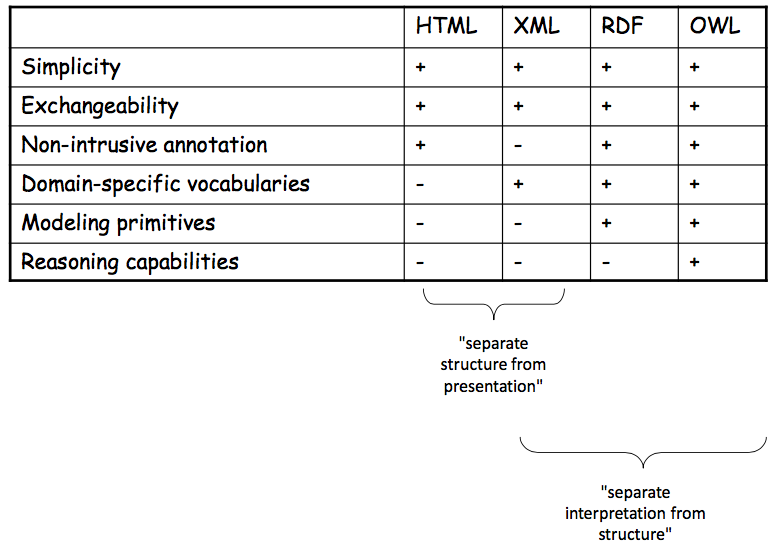
\includegraphics[width=1\linewidth]{figures/ontology.png}
\end{center}
\caption{Model Requirements for Ontologies}
\end{figure}


\subsection{RDF -- Resource Description Framework}

\paragraph{RDF} is a standard supported by the W3C to represent metadata

RDF consists of two part:
\begin{enumerate}
\item language for representing metadata instance, which allow to annotate web resources with statement
\item a language for specifying schemas for RDF instance. Define grammar and vocabulary for semantic domain
\end{enumerate}

RDF statement can be represented as a:
\begin{itemize}
\item Statement where the subject is an URI (uniform resource identifier) and object is a URI or string
\item Directed graph: the subject and object are represented as nodes (ellipses for resources and rectangles for literal and predicate as directed link)
\item XML Documents: encoded into XML
\end{itemize}

\subsubsection{RDF syntax}
\begin{figure}[H]
\begin{center}
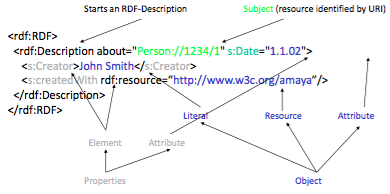
\includegraphics[width=1\linewidth]{figures/rdf.png}
\end{center}
\caption{RDF syntax}
\end{figure}

\paragraph{Typing resources:} resources can be categorize into different classes/type by using \bf{rdf:type}. We can abbreviate the syntax where the name of the type becomes the element name of the element representing the statement

\begin{figure}[H]
\begin{center}
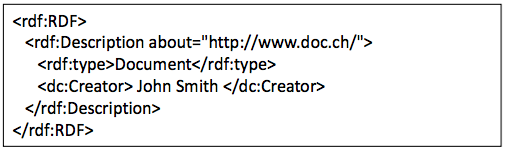
\includegraphics[width=1\linewidth]{figures/type.png}
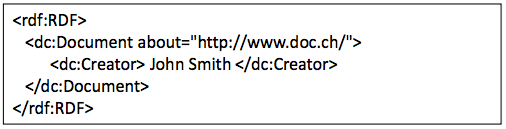
\includegraphics[width= 1\linewidth]{figures/abbr.png}
\end{center}
\caption{\textit{top:}RDF syntax with type, \textit{down:}abbreviated syntax}
\end{figure}

\paragraph{RDF complex value:} sometimes a property may be a complex statement. In order to represent such complex value, a new intermediate resource is created to which different properties are associated

\begin{figure}[H]
\begin{center}
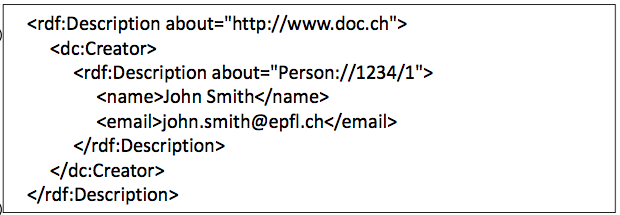
\includegraphics[width=1\linewidth]{figures/complexRDF.png}
\end{center}
\caption{Example of a RDF complex value}
\end{figure}

\paragraph{RDF containers}statement can be made not only using single resources but  as well using collections of resources. Container are special resources of one or three container types that are specified in the RDF standard:

\begin{itemize}
\item Bag: unordered multi-set (= sets with multiple occurrence of the same resources)
\item Seq: ordered set (list)
\item Alt: alternative (a single resource that is to be chosen out of the given set)
\end{itemize}

\begin{figure}[H]
\begin{center}
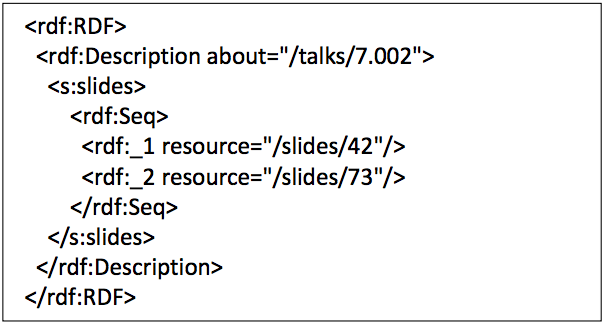
\includegraphics[width=1\linewidth]{figures/container.png}
\end{center}
\caption{Example of a containers (seq)}
\end{figure}

\paragraph{Creating new Resources:} RDF resources need not necessarily be a pre-existing Web
resources identified by URIs, but can also be instantiated within RDF statement. \bf{rdf:ID}
replaces \bf{rdf:about} when the statement is about a new resources instead of an existing one or
use rdf:about = ``\#\dots'' e.g. rdf:ID=``12345'' = rdf:about = ``\#12345''

\paragraph{RDF Reification:} everything is a resource, RDF statements are also considered as resources and therefore it should be possible to make statements about them. We introduce a new resource which serves as representative for the statement. This resource obtains as properties all the constituent that make up the statement it represents. It is called \bf{reification}. The type of the object can be determined through a property \textit{rdf:type} pointing to the special resource \textit{rdf:statement} representing the category of statement. For the predicate a specific new resource representing the predicate is require

\begin{figure}[H]
\begin{center}
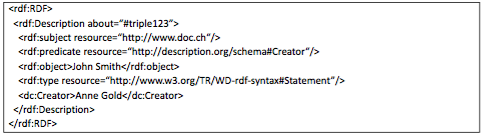
\includegraphics[width=1\linewidth]{figures/reification.png}
\end{center}
\caption{Example of a reification)}
\end{figure}

\subsubsection{RDF Schema}

\paragraph{Classes} are represented themselves as resources, which are of type \bf{rdfs:Class}. The \textit{rdf:type} is then used to indicate the type of a class resource. between classes a subclass relationship can be specified by using \bf{rdfs:subclass}

In RDF everything is a resource. In particular $classes$ are sets of $resources$ and thus \textit{rdfs:Class} is a subclass of \textit{rdfs:Resource}. But since \textit{rdfs:Resource} is a class, it is connected via the \textit{rdf:Type} to the \textit{rdf:Class} resource. This produce a cyclic structure (see Figure \ref{fig:class})

\begin{figure}[H]
\begin{center}
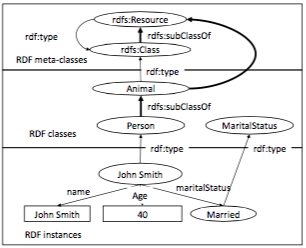
\includegraphics[width=1\linewidth]{figures/class.png}
\end{center}
\caption{Classification}
\label{fig:class}
\end{figure}

\paragraph{Properties:} it is possible to constrain the usage of RDF properties that connect resources as follows: by connecting the property resource through the property \textit{rdfs:domain} to a class resource, one specifies that the subject when using this property must be of the type of this class. We can also constrain the range using \textit{rdfs:range}

\begin{figure}[H]
\begin{center}
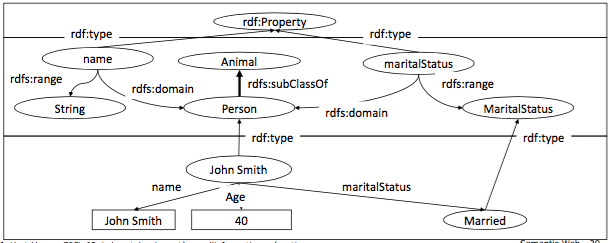
\includegraphics[width=1\linewidth]{figures/properties.png}
\end{center}
\caption{Properties}
\label{fig:class}
\end{figure}

\paragraph{RDF Schema Inheritance}
\begin{itemize}
	\item \bf{rdfs:subClassOf:}
		\begin{itemize}
			\item $A$ subClassOf $B$: Every instance of $A$ is also instance of $B$
			\item Properties are transitive, not reflexive, anti-symmetric (no cycles!),
			\item M:N: a class can have arbitrarily many subclasses and superclasses
			\item Subclass has all properties of the superclass
		\end{itemize}
	\item \bf{rdfs:subPropertyOf}
		\begin{itemize}
			\item $P1$ subPropertyOf $P2$: If $A$ has Property $P1$ with value $B$ then it has also value $B$ with Property $P2$
			\item Example: Anne has Property Father with value John, and Father subProperty AParent implies Anne has Property AParent with value John
		\end{itemize}
\end{itemize}

\begin{figure}[H]
\begin{center}
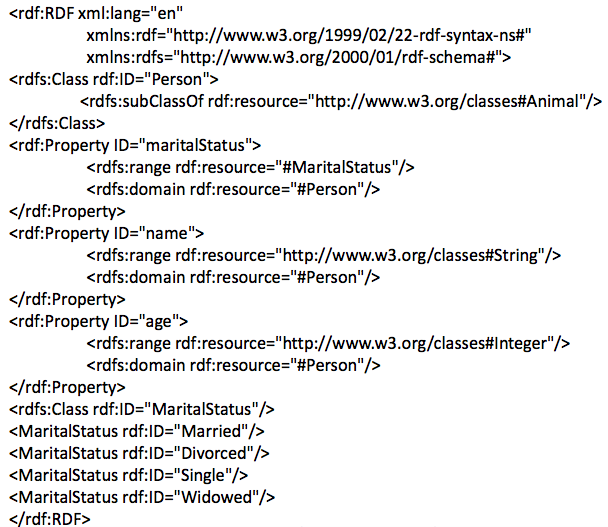
\includegraphics[width=1\linewidth]{figures/rdf_syntax.png}
\end{center}
\caption{Syntax all together}
\label{fig:class}
\end{figure}

\subsection{OWL - Ontology Languages}
Limitation of RDF Schema:
\begin{itemize}
	\item Limited expressive power (sublcass, property, subproperty)
	\item Unclear semantics (e.g. subpropertiy never has been precisely defined) it is therefore, for example, not always possible to decide whether a given RDF instance corresponds to a given schema
	\item No reasoning support
\end{itemize}

Requirement on ontology languages:
\begin{itemize}
	\item well \bf{designed}: intuitive to human user, adequate expressive power
	\item well \bf{defined}: clearly specified syntax, formal semantics, adequate expressive power
	\item \bf{Compatible} with existing (web) standards: in particular RDV
\end{itemize}

\subsubsection{OWL (Web Ontology Language)}
The language to specify OWL models is given as an RDF Schema
\begin{itemize}
	\item like the RDF schema language is expressed within an RDF schema
	\item therefore OWL models can be expressed in RDF
	\item some of the OWL modelling primitives and RDF modelling primitives overlap and are re-used in OWL 
\end{itemize}

\begin{figure}[H]
\begin{center}
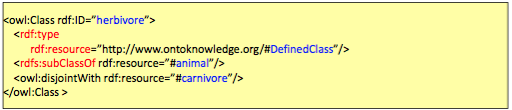
\includegraphics[width=1\linewidth]{figures/owl.png}
\end{center}
\caption{OWL}
\end{figure}

The semantics of OWL is given in \bf{Description Logics (DL)}. 
\begin{itemize}
	\item Description logic is a sublanguage of first order predicate logic. 
	\item reasoning (deriving/proving statement) can be done more efficiently than in first order predicate logic
\end{itemize}



Class in OWL are \textit{unary} predicate. Slot constraint (= properties) in OWL are \textit{binary predicate}

\begin{figure}[H]
\begin{center}
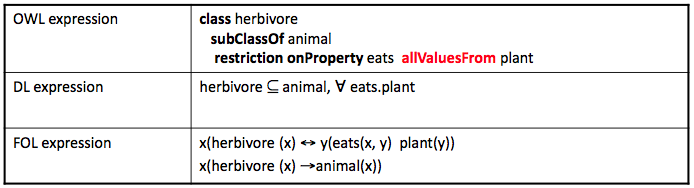
\includegraphics[width=1\linewidth]{figures/semantic_owl.png}
\end{center}
\caption{OWL semantic}
\end{figure}

\begin{figure}[H]
\begin{center}
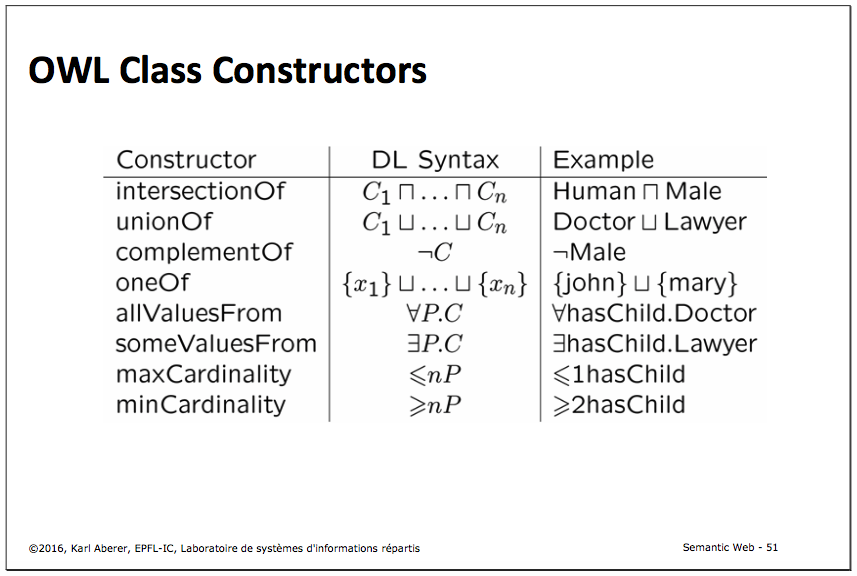
\includegraphics[width=1\linewidth]{figures/owl_class.png}
\end{center}
\caption{OWL class constructor}
\end{figure}

\begin{figure}[H]
\begin{center}
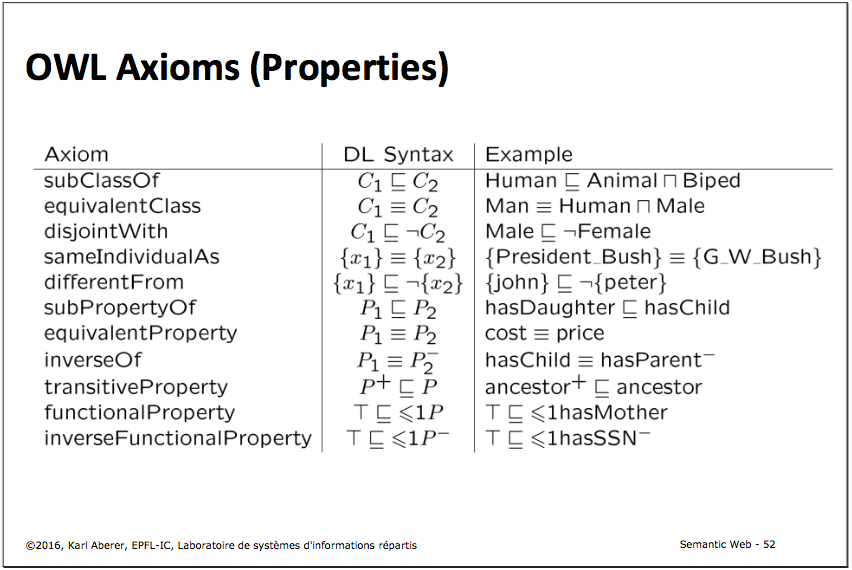
\includegraphics[width=1\linewidth]{figures/owl_axioms.png}
\end{center}
\caption{OWL axioms}
\end{figure}


\subsection{Semantic Web Resources}
Example of popular concrete ontologies: WordNet, Schema.org, WikiData, Google Knowledge Graph, Linked Open Data

(The description of each ontology doesn't seem very relevant for the exam)
